\documentclass[11pt, a4paper]{article}
%\usepackage{proj1}
\usepackage{natbib}
\usepackage{fancyhdr}  
\usepackage{subcaption}
\usepackage{caption}
\usepackage{graphicx}
\usepackage{numprint}
\usepackage{multirow}
\linespread{1.25} 
\setlength{\parindent}{0cm}
\graphicspath{{Images/}}
\usepackage{hyperref}
\usepackage{amsmath}
\usepackage{amsfonts}
\usepackage{amssymb}
\usepackage{amsthm}
\usepackage{mathtools}
\usepackage{commath}
\usepackage{bbm}

%\usepackage[sc,osf]{mathpazo}
\usepackage{subcaption}
\usepackage[a4paper, top=1in, left=1.0in, right=1.0in, bottom=1in, includehead, includefoot]{geometry} %Usually have top as 1in

\usepackage{listings}
\usepackage{color} %red, green, blue, yellow, cyan, magenta, black, white
\definecolor{mygreen}{RGB}{28,172,0} % color values Red, Green, Blue
\definecolor{mylilas}{RGB}{170,55,241}


\hypersetup{colorlinks,linkcolor={black},citecolor={blue},urlcolor={black}}
\usepackage{color}
\urlstyle{same}


\theoremstyle{definition}
\newtheorem{definition}{Definition}[section]

\newcommand{\adja}{q_a}
\newcommand{\adjb}{q_b}
\newcommand{\adjaB}{q_{a,\partial \Omega}}
\newcommand{\adjbB}{q_{b,\partial \Omega}}
\newcommand{\adjB}{q_{\partial \Omega}}
\newcommand{\Adja}{\mathbf{p}}
\newcommand{\Adjb}{q}
\newcommand{\adj}{q}
\newcommand{\Adjc}{{q}_{\partial \Omega}}
\newcommand{\ra}{\rho_a}
\newcommand{\rb}{\rho_b}
\newcommand{\w}{\mathbf{w}}
\newcommand{\f}{\mathbf{f}}
\newcommand{\ve}{\mathbf{v}}
\newcommand{\n}{\mathbf{n}}
\newcommand{\h}{\mathbf{h}}
\newcommand{\K}{\mathbf{K}}
\newcommand{\hr}{\widehat \rho}

%	\begin{figure}[h]
%		\centering
%		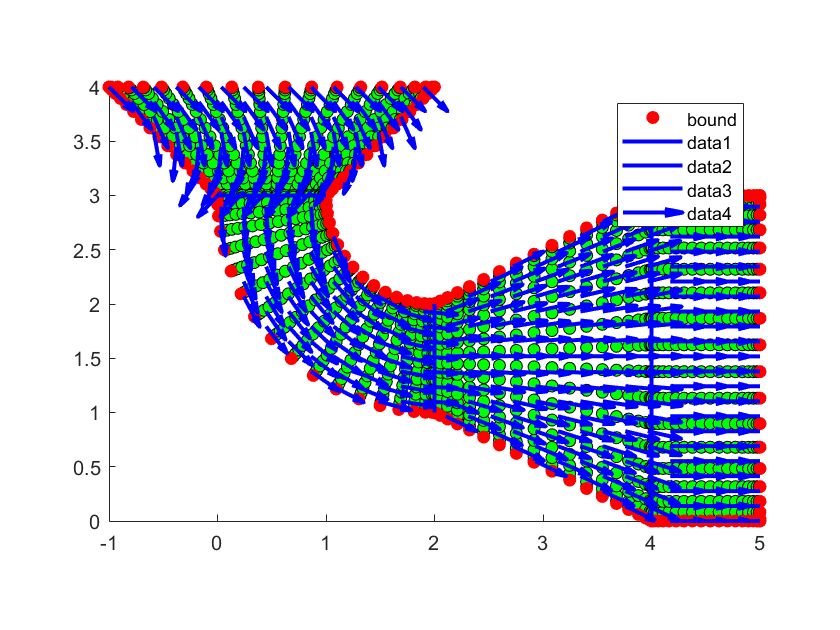
\includegraphics[scale=0.35]{F1.png}
%		\caption{Forward $\rho$ for $a = 0.01$} 
%		\label{F1}
%	\end{figure}

\begin{document}
	
	\section{Averaging the advection-diffusion equation}
	We consider the standard advection-diffusion optimality system, with flow control and Neumann boundary conditions:
	\begin{align*}
		\frac{\partial \rho}{\partial t} &= \nabla^2 \rho - \nabla \cdot (\rho \w) + f\\
		0 &= (- \nabla \rho + \rho \w) \cdot \n \\
		\\
		\frac{\partial q}{\partial t} &= - \nabla^2 q - \w \cdot \nabla q - \rho + \hr\\
		0 &= \nabla q \cdot \n \\
		\\
		\w &= - \frac{1}{\beta}\rho \nabla q
	\end{align*}
	We now have the following operators in polar coordinates acting on a function $f$ and a vector field $\w$:
	\begin{align*}
		\nabla^2 f &= \frac{1}{r} \frac{\partial}{\partial r} \left( r \frac{\partial f}{\partial r}\right) + \frac{1}{r^2} \frac{\partial^2 f}{\partial \theta^2} + \frac{\partial f}{\partial z^2}\\
		\nabla f &= \left(\frac{\partial f}{\partial r}, \frac{1}{r}\frac{\partial f}{\partial \theta}, \frac{\partial f}{\partial z}\right)\\
		\nabla \cdot \w &= \frac{1}{r}\frac{\partial }{\partial r}\left(r \w_r\right) - \frac{1}{r}\frac{\partial \w_\theta}{\partial \theta} + \frac{\partial \w_z}{\partial z}
	\end{align*}
	Implementing these, we get:
	\begin{align*}
		\frac{\partial \rho}{\partial t} &= \frac{1}{r} \frac{\partial}{\partial r} \left( r \frac{\partial \rho}{\partial r}\right) + \frac{1}{r^2} \frac{\partial^2 \rho}{\partial \theta^2} + \frac{\partial \rho}{\partial z^2} - \frac{1}{r}\frac{\partial }{\partial r}\left(r \rho\w_r\right) + \frac{1}{r}\frac{\partial \rho\w_\theta}{\partial \theta} - \frac{\partial \rho\w_z}{\partial z} + f\\
		0 &= \left(- \left(\frac{\partial \rho}{\partial r}, \frac{1}{r}\frac{\partial \rho}{\partial \theta}, \frac{\partial \rho}{\partial z}\right) + \rho \w \right) \cdot \n \\
		\\
		\frac{\partial q}{\partial t} &= -  \frac{1}{r} \frac{\partial}{\partial r} \left( r \frac{\partial q}{\partial r}\right) - \frac{1}{r^2} \frac{\partial^2 fq}{\partial \theta^2} - \frac{\partial q}{\partial z^2} - \w \cdot \left(\frac{\partial q}{\partial r}, \frac{1}{r}\frac{\partial q}{\partial \theta}, \frac{\partial q}{\partial z}\right) - \rho + \hr\\
		0 &= \left(\frac{\partial q}{\partial r}, \frac{1}{r}\frac{\partial q}{\partial \theta}, \frac{\partial q}{\partial z}\right) \cdot \n \\
		\\
		\w &= - \frac{1}{\beta}\rho  \left(\frac{\partial q}{\partial r}, \frac{1}{r}\frac{\partial q}{\partial \theta}, \frac{\partial q}{\partial z}\right)
	\end{align*}
	Then we set $\theta$ to be constant, so that all derivatives in $\theta$ are zero and we multiply out some derivatives, to get:
	
		\begin{align*}
		\frac{\partial \rho}{\partial t} &= \frac{1}{r} \frac{\partial \rho}{\partial r} +  \frac{\partial^2 \rho}{\partial r^2} + \frac{\partial \rho}{\partial z^2} - \frac{\rho\w_r}{r} -\rho\frac{\partial \w_r }{\partial r} -\w_r\frac{\partial \rho}{\partial r} - \rho\frac{\partial \w_z}{\partial z}- \w_z\frac{\partial \rho}{\partial z} + f\\
		0 &= \left(- \left(\frac{\partial \rho}{\partial r},  \frac{\partial \rho}{\partial z}\right) + \rho \w \right) \cdot \n \\
		\\
		\frac{\partial q}{\partial t} &= - \frac{1}{r} \frac{\partial q}{\partial r} -  \frac{\partial^2 q}{\partial r^2} - \frac{\partial q}{\partial z^2} - \w \cdot \left(\frac{\partial q}{\partial r},  \frac{\partial q}{\partial z}\right) - \rho + \hr\\
		0 &= \left(\frac{\partial q}{\partial r},  \frac{\partial q}{\partial z}\right) \cdot \n \\
		\\
		\w &= - \frac{1}{\beta}\rho  \left(\frac{\partial q}{\partial r},  \frac{\partial q}{\partial z}\right)
	\end{align*}
	We can rewrite some of the terms in the forward equation:
	\begin{align*}
		-\w_r\frac{\partial \rho}{\partial r} - \w_z\frac{\partial \rho}{\partial z} &= - \left(\w \cdot \nabla \right)\rho\\
		-\rho\frac{\partial \w_r }{\partial r} - \rho\frac{\partial \w_z}{\partial z} &= -\left(\nabla \cdot \w \right)\rho 
	\end{align*}
	Using the vector identity $\mathbf a (\nabla \cdot \mathbf b) + (\mathbf b \cdot \nabla ) \mathbf a = \nabla \cdot (\mathbf{b a^T})$, we get that the above two terms become:
	\begin{align*}
		- \left(\w \cdot \nabla \right)\rho - \left(\nabla \cdot \w \right)\rho = - \nabla \cdot (\rho\w ).
	\end{align*}
	
	Then the optimality system is:
	\begin{align*}
		\frac{\partial \rho}{\partial t} &= \frac{1}{r} \frac{\partial \rho}{\partial r} +  \frac{\partial^2 \rho}{\partial r^2} + \frac{\partial \rho}{\partial z^2} - \frac{\rho\w_r}{r} - \nabla \cdot (\rho \w ) + f\\
		0 &= \left(- \left(\frac{\partial \rho}{\partial r},  \frac{\partial \rho}{\partial z}\right) + \rho \w \right) \cdot \n \\
		\\
		\frac{\partial q}{\partial t} &= - \frac{1}{r} \frac{\partial q}{\partial r} -  \frac{\partial^2 q}{\partial r^2} - \frac{\partial q}{\partial z^2} - \w \cdot \left(\frac{\partial q}{\partial r},  \frac{\partial q}{\partial z}\right) - \rho + \hr\\
		0 &= \left(\frac{\partial q}{\partial r},  \frac{\partial q}{\partial z}\right) \cdot \n \\
		\\
		\w &= - \frac{1}{\beta}\rho  \left(\frac{\partial q}{\partial r},  \frac{\partial q}{\partial z}\right)
	\end{align*}
	
	\subsection{Exact Solution}
	We are choosing an exact solution which satisfies the boundary conditions, matches the final time condition for $q$ and is invariant in $\theta$. We choose:
	\begin{align*}
		\rho &= \beta^{1/2} e^t \cos(\pi r) \cos (\pi z)\\
		q &= \beta^{1/2}(e^T - e^t)\cos(\pi r)\cos(\pi z),
	\end{align*}
	and use these to determine the values of $\w$, $f$ and $\hr$.
	\\
	\\
	There must be a mistake somewhere because the exact solution is still not exact. I am not sure what this mistake is yet.
	
	\section{Sedimentation Equation Papers}
	The paper Archer cites for the form of the free energy functional is by Yaakov Rosenfeld and is called 'Free-energy model for the inhomogeneous hard-sphere fluid in D dimensions:
	Structure factors for the hard-disk (D =2) mixtures in simple explicit form'.
	I cannot seem to link an equation directly to the one in Archer's paper. There is one that looks sort of similar, which is equation (4.11):
	\begin{align*}
		\Phi = - n_0 \ln (1-n_2) + \frac{1}{4 \pi} \frac{n_1 n_1}{1-n_2} +  \frac{1}{4 \pi} \frac{\mathbf{n_1 n_1}}{1-n_2}.
	\end{align*}
	The one in Archer's paper is:
	\begin{align*}
		F = \rho \left(\ln(\Lambda^2 \rho) -2 -\ln(1-a\rho) + \frac{1}{1-a\rho}\right), 
	\end{align*}
	where $a = \pi \sigma^2 /4$.
	\\
	We were thinking about doing the averaging with the sedimentation stuff. Is this equation valid for 3D?
	
	\section{Periodic Boundary Conditions}
	We consider the advection diffusion equation with periodic boundary conditions and a corresponding OCP:
	\begin{align*}
		&\min \frac{1}{2}|| \rho - \hr||^2 + \frac{\beta}{2}||\w||^2\\
		&\text{subject to:}\\
		&\frac{\partial \rho}{\partial t} = \frac{\partial^2 \rho}{\partial x^2} - \frac{\partial \rho \w}{\partial x}\\
		& \rho(a) = \rho(b)\\
		& \frac{\partial \rho(a)}{\partial x} = \frac{\partial \rho(b)}{\partial x} 
	\end{align*}
	The relevant part of the Lagrangian is then:
	\begin{align*}
		\mathcal{L} = ... -\int_0^T \int_\Omega \left(\frac{\partial \rho}{\partial t} - \frac{\partial^2 \rho}{\partial x^2} + \frac{\partial \rho \w}{\partial x}\right)q dr dt - \int_0^T \left(\rho(b) - \rho(a) + \frac{\partial \rho(b)}{\partial x} - \frac{\partial \rho(a)}{\partial x}\right)q_2dt.
	\end{align*}
	Taking partial derivatives, the relevant part of the Lagrangian is:
	\begin{align*}
		\mathcal{L} = ... - \int_0^T \left[q \frac{\partial \rho}{\partial x} - \rho\frac{\partial q}{\partial x} - \rho \w q\right]_a^b +
		\left(\rho(b) - \rho(a) + \frac{\partial \rho(b)}{\partial x} - \frac{\partial \rho(a)}{\partial x}\right)q_2dt.
	\end{align*}
	Taking the derivative with respect to $\rho$ gives:
	\begin{align*}
		\mathcal{L}_\rho h = ... - \int_0^T \left[q \frac{\partial h}{\partial x} - h\frac{\partial q}{\partial x} - h \w q\right]_a^b -
		\left(h(b) - h(a) + \frac{\partial h(b)}{\partial x} - \frac{\partial h(a)}{\partial x}\right)q_2dt
	\end{align*}
	Rewriting the second bracket so it matches the first gives:
	\begin{align*}
		\mathcal{L}_\rho h = ... - \int_0^T \left[q \frac{\partial h}{\partial x} - h\frac{\partial q}{\partial x} - h \w q - h q_2 - \frac{\partial h}{\partial x}q_2 \right]_a^b dt
	\end{align*}
	Considering $h = 0$ and $\frac{\partial h}{\partial x} \neq 0$, we get that $q = q_2$.
	Then considering $h \neq 0$ we see that:
	\begin{align*}
		\left[ - \frac{\partial q}{\partial x} -  \w q -  q_2  \right]_a^b = 0.
	\end{align*}
	And since $q_2 = q$, we have:
	\begin{align*}
		\left[ - \frac{\partial q}{\partial x} -  \w q -  q  \right]_a^b = 0.
	\end{align*}
	This seems close but isn't quite right. I am also not sure how to separate the individual boundary conditions again.
	
	\section{Varying Flow Problem Setup}
	I have created a multishape with varying flows. For this I wanted to adapt the fancy channel code by rotating one of the trapezia by 90 degrees. Somehow this doesn't seem to be working. In Figure \ref{F1a} the multishape with flow is shown. In Figure \ref{F1b} on the left the code for the flow of shape one is shown, which isn't quite working and on the right the code for the flow of shape three is shown, which is working.
	
		\begin{figure}[h]
			\centering
			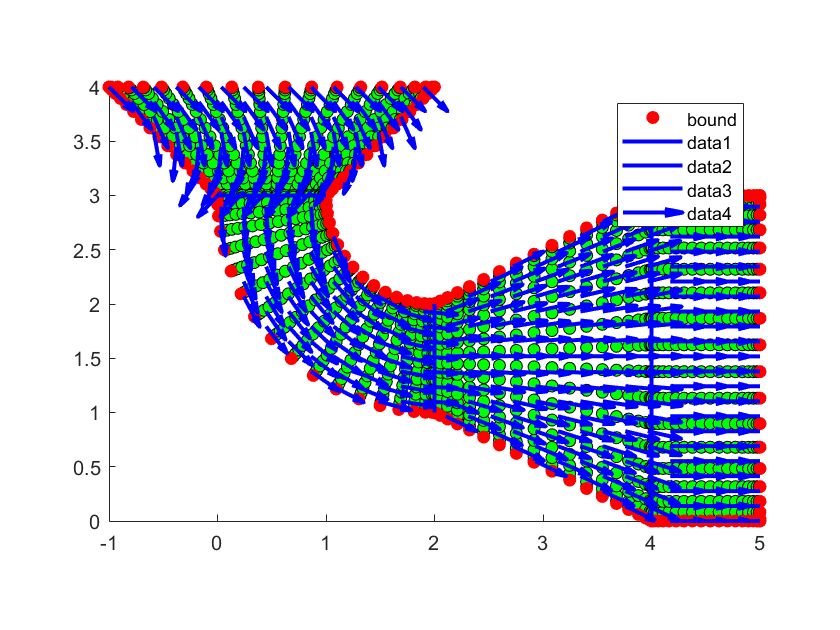
\includegraphics[scale=0.5]{F1.png}
			\caption{Multishape with flow} 
			\label{F1a}
		\end{figure}
		\begin{figure}[h]
			\centering
			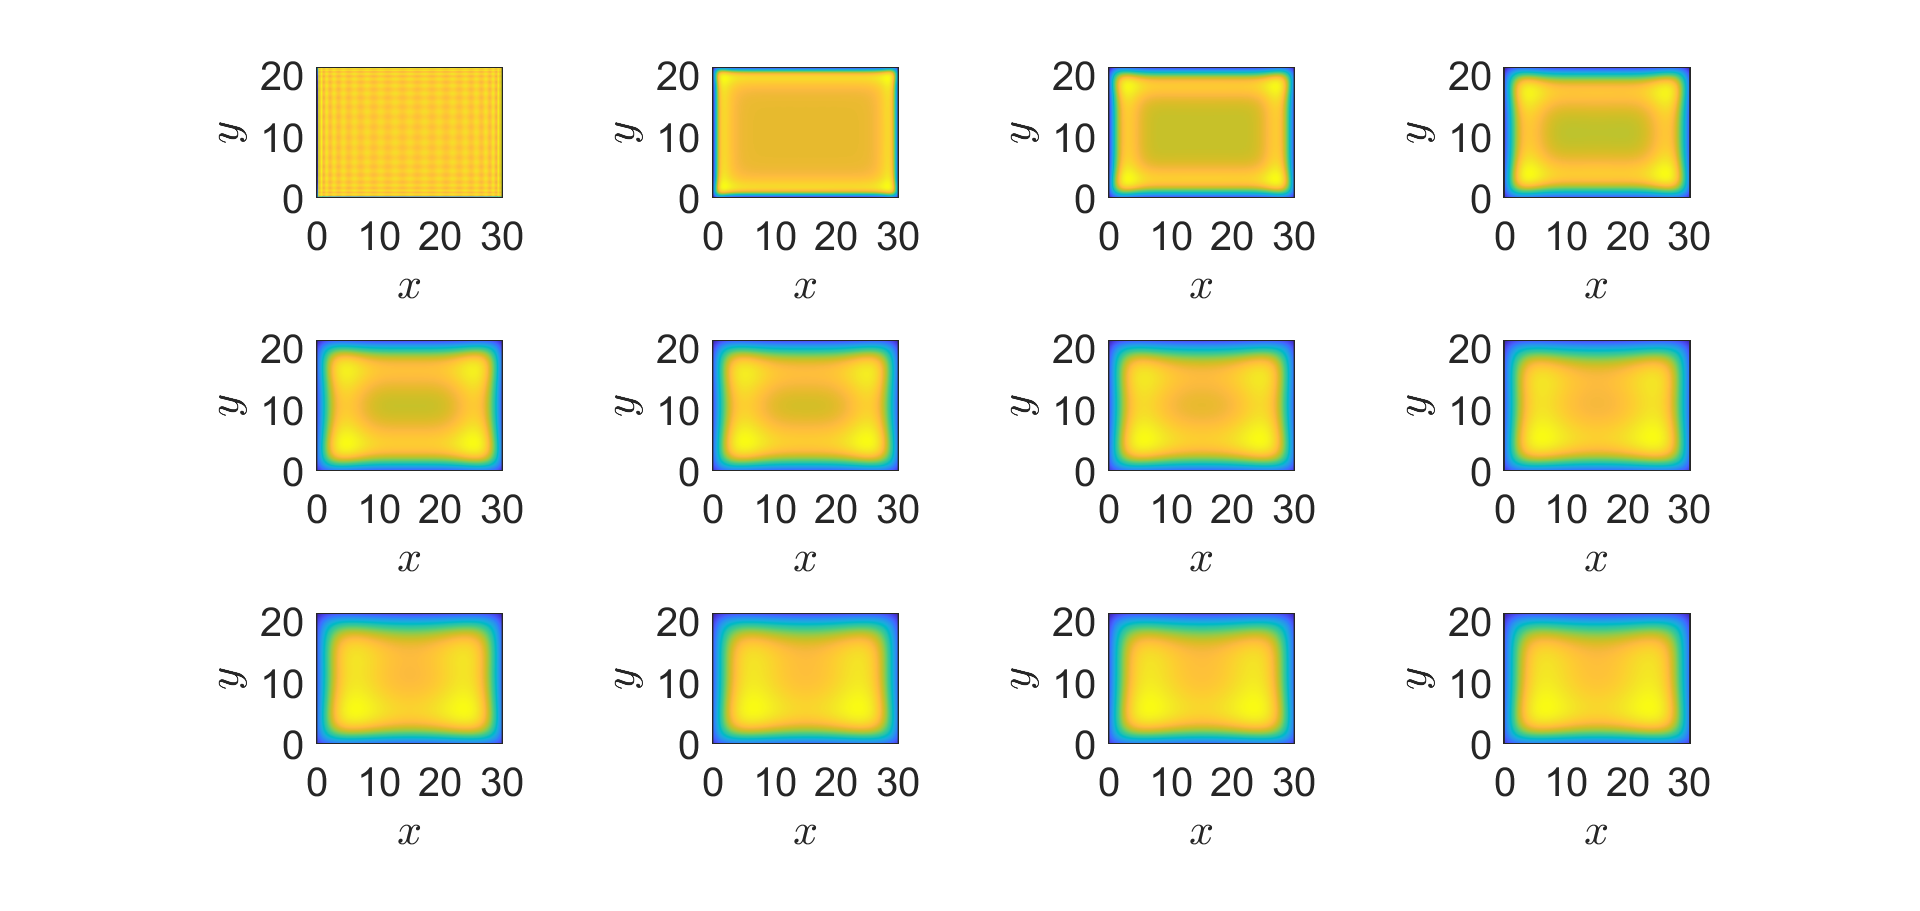
\includegraphics[scale=0.6]{C1.png}
			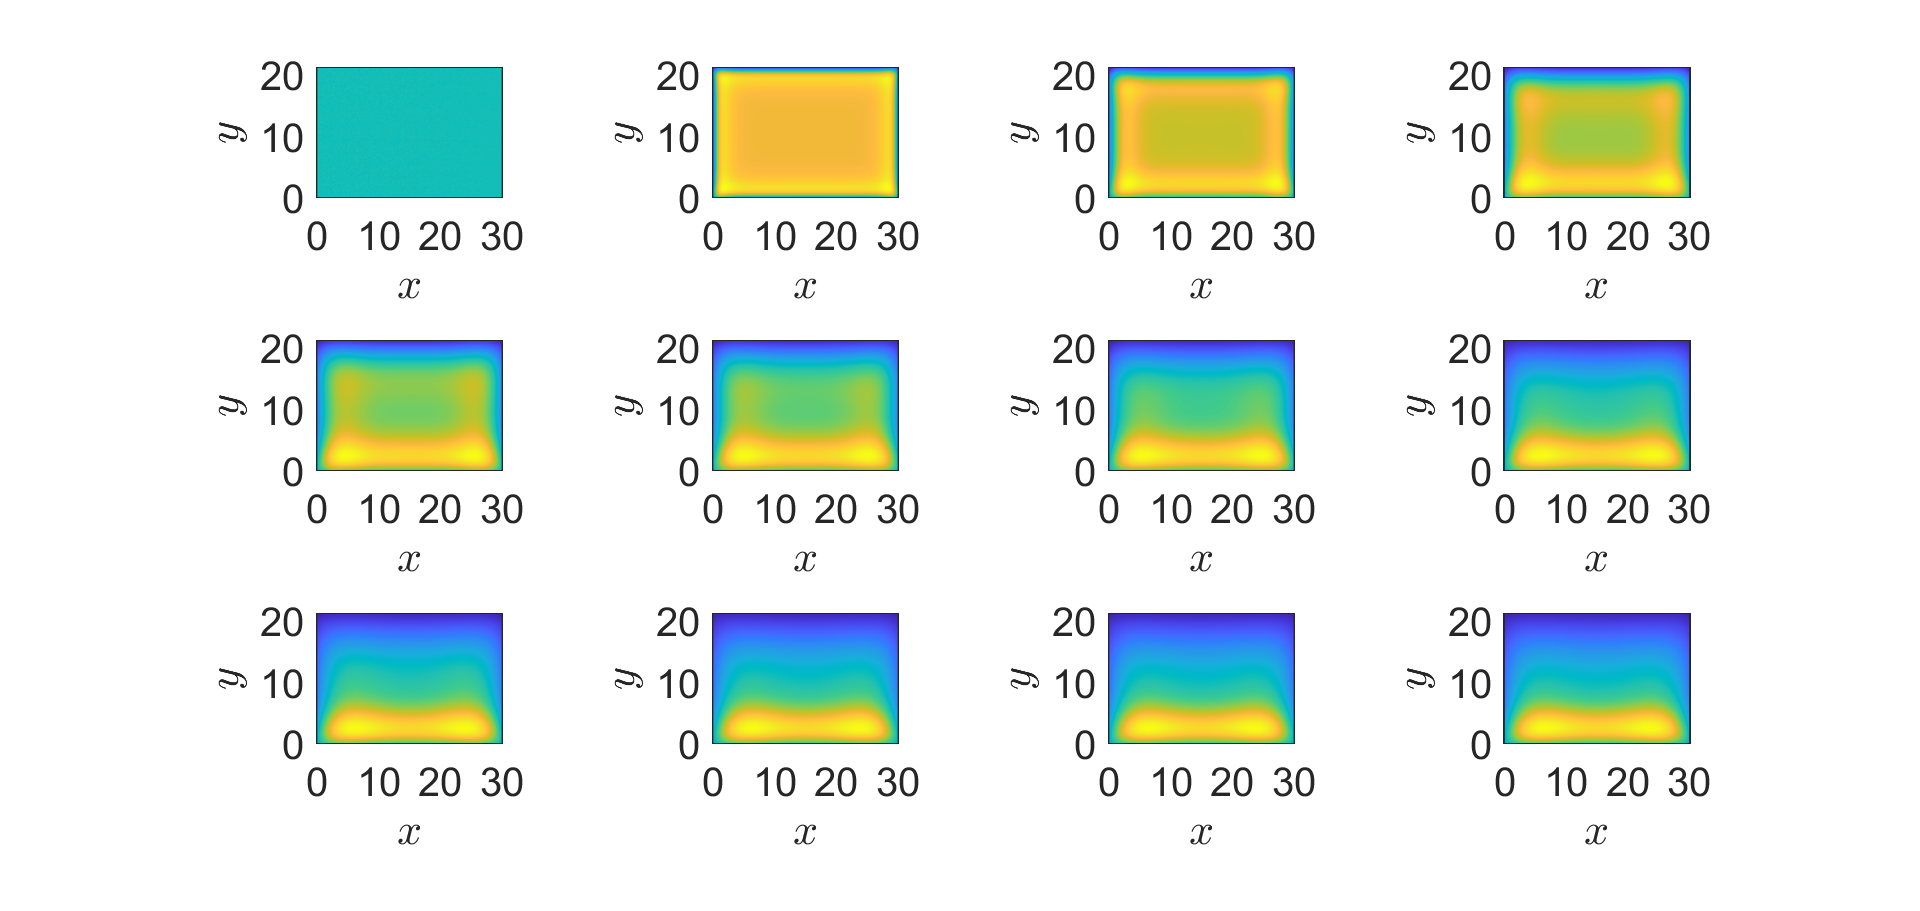
\includegraphics[scale=0.6]{C2.png}
			\caption{Code for shape 1 and shape 3} 
			\label{F1b}
		\end{figure}
	
	
\end{document}